% Options for packages loaded elsewhere
\PassOptionsToPackage{unicode}{hyperref}
\PassOptionsToPackage{hyphens}{url}
%
\documentclass[
]{book}
\usepackage{amsmath,amssymb}
\usepackage{lmodern}
\usepackage{iftex}
\ifPDFTeX
  \usepackage[T1]{fontenc}
  \usepackage[utf8]{inputenc}
  \usepackage{textcomp} % provide euro and other symbols
\else % if luatex or xetex
  \usepackage{unicode-math}
  \defaultfontfeatures{Scale=MatchLowercase}
  \defaultfontfeatures[\rmfamily]{Ligatures=TeX,Scale=1}
\fi
% Use upquote if available, for straight quotes in verbatim environments
\IfFileExists{upquote.sty}{\usepackage{upquote}}{}
\IfFileExists{microtype.sty}{% use microtype if available
  \usepackage[]{microtype}
  \UseMicrotypeSet[protrusion]{basicmath} % disable protrusion for tt fonts
}{}
\makeatletter
\@ifundefined{KOMAClassName}{% if non-KOMA class
  \IfFileExists{parskip.sty}{%
    \usepackage{parskip}
  }{% else
    \setlength{\parindent}{0pt}
    \setlength{\parskip}{6pt plus 2pt minus 1pt}}
}{% if KOMA class
  \KOMAoptions{parskip=half}}
\makeatother
\usepackage{xcolor}
\usepackage{color}
\usepackage{fancyvrb}
\newcommand{\VerbBar}{|}
\newcommand{\VERB}{\Verb[commandchars=\\\{\}]}
\DefineVerbatimEnvironment{Highlighting}{Verbatim}{commandchars=\\\{\}}
% Add ',fontsize=\small' for more characters per line
\usepackage{framed}
\definecolor{shadecolor}{RGB}{248,248,248}
\newenvironment{Shaded}{\begin{snugshade}}{\end{snugshade}}
\newcommand{\AlertTok}[1]{\textcolor[rgb]{0.94,0.16,0.16}{#1}}
\newcommand{\AnnotationTok}[1]{\textcolor[rgb]{0.56,0.35,0.01}{\textbf{\textit{#1}}}}
\newcommand{\AttributeTok}[1]{\textcolor[rgb]{0.77,0.63,0.00}{#1}}
\newcommand{\BaseNTok}[1]{\textcolor[rgb]{0.00,0.00,0.81}{#1}}
\newcommand{\BuiltInTok}[1]{#1}
\newcommand{\CharTok}[1]{\textcolor[rgb]{0.31,0.60,0.02}{#1}}
\newcommand{\CommentTok}[1]{\textcolor[rgb]{0.56,0.35,0.01}{\textit{#1}}}
\newcommand{\CommentVarTok}[1]{\textcolor[rgb]{0.56,0.35,0.01}{\textbf{\textit{#1}}}}
\newcommand{\ConstantTok}[1]{\textcolor[rgb]{0.00,0.00,0.00}{#1}}
\newcommand{\ControlFlowTok}[1]{\textcolor[rgb]{0.13,0.29,0.53}{\textbf{#1}}}
\newcommand{\DataTypeTok}[1]{\textcolor[rgb]{0.13,0.29,0.53}{#1}}
\newcommand{\DecValTok}[1]{\textcolor[rgb]{0.00,0.00,0.81}{#1}}
\newcommand{\DocumentationTok}[1]{\textcolor[rgb]{0.56,0.35,0.01}{\textbf{\textit{#1}}}}
\newcommand{\ErrorTok}[1]{\textcolor[rgb]{0.64,0.00,0.00}{\textbf{#1}}}
\newcommand{\ExtensionTok}[1]{#1}
\newcommand{\FloatTok}[1]{\textcolor[rgb]{0.00,0.00,0.81}{#1}}
\newcommand{\FunctionTok}[1]{\textcolor[rgb]{0.00,0.00,0.00}{#1}}
\newcommand{\ImportTok}[1]{#1}
\newcommand{\InformationTok}[1]{\textcolor[rgb]{0.56,0.35,0.01}{\textbf{\textit{#1}}}}
\newcommand{\KeywordTok}[1]{\textcolor[rgb]{0.13,0.29,0.53}{\textbf{#1}}}
\newcommand{\NormalTok}[1]{#1}
\newcommand{\OperatorTok}[1]{\textcolor[rgb]{0.81,0.36,0.00}{\textbf{#1}}}
\newcommand{\OtherTok}[1]{\textcolor[rgb]{0.56,0.35,0.01}{#1}}
\newcommand{\PreprocessorTok}[1]{\textcolor[rgb]{0.56,0.35,0.01}{\textit{#1}}}
\newcommand{\RegionMarkerTok}[1]{#1}
\newcommand{\SpecialCharTok}[1]{\textcolor[rgb]{0.00,0.00,0.00}{#1}}
\newcommand{\SpecialStringTok}[1]{\textcolor[rgb]{0.31,0.60,0.02}{#1}}
\newcommand{\StringTok}[1]{\textcolor[rgb]{0.31,0.60,0.02}{#1}}
\newcommand{\VariableTok}[1]{\textcolor[rgb]{0.00,0.00,0.00}{#1}}
\newcommand{\VerbatimStringTok}[1]{\textcolor[rgb]{0.31,0.60,0.02}{#1}}
\newcommand{\WarningTok}[1]{\textcolor[rgb]{0.56,0.35,0.01}{\textbf{\textit{#1}}}}
\usepackage{longtable,booktabs,array}
\usepackage{calc} % for calculating minipage widths
% Correct order of tables after \paragraph or \subparagraph
\usepackage{etoolbox}
\makeatletter
\patchcmd\longtable{\par}{\if@noskipsec\mbox{}\fi\par}{}{}
\makeatother
% Allow footnotes in longtable head/foot
\IfFileExists{footnotehyper.sty}{\usepackage{footnotehyper}}{\usepackage{footnote}}
\makesavenoteenv{longtable}
\usepackage{graphicx}
\makeatletter
\def\maxwidth{\ifdim\Gin@nat@width>\linewidth\linewidth\else\Gin@nat@width\fi}
\def\maxheight{\ifdim\Gin@nat@height>\textheight\textheight\else\Gin@nat@height\fi}
\makeatother
% Scale images if necessary, so that they will not overflow the page
% margins by default, and it is still possible to overwrite the defaults
% using explicit options in \includegraphics[width, height, ...]{}
\setkeys{Gin}{width=\maxwidth,height=\maxheight,keepaspectratio}
% Set default figure placement to htbp
\makeatletter
\def\fps@figure{htbp}
\makeatother
\setlength{\emergencystretch}{3em} % prevent overfull lines
\providecommand{\tightlist}{%
  \setlength{\itemsep}{0pt}\setlength{\parskip}{0pt}}
\setcounter{secnumdepth}{5}
\usepackage{booktabs}
\ifLuaTeX
  \usepackage{selnolig}  % disable illegal ligatures
\fi
\usepackage[]{natbib}
\bibliographystyle{plainnat}
\IfFileExists{bookmark.sty}{\usepackage{bookmark}}{\usepackage{hyperref}}
\IfFileExists{xurl.sty}{\usepackage{xurl}}{} % add URL line breaks if available
\urlstyle{same} % disable monospaced font for URLs
\hypersetup{
  pdftitle={MEPS tutorials},
  pdfauthor={Mark Bounthavong},
  hidelinks,
  pdfcreator={LaTeX via pandoc}}

\title{MEPS tutorials}
\author{Mark Bounthavong}
\date{2023-07-22}

\usepackage{amsthm}
\newtheorem{theorem}{Theorem}[chapter]
\newtheorem{lemma}{Lemma}[chapter]
\newtheorem{corollary}{Corollary}[chapter]
\newtheorem{proposition}{Proposition}[chapter]
\newtheorem{conjecture}{Conjecture}[chapter]
\theoremstyle{definition}
\newtheorem{definition}{Definition}[chapter]
\theoremstyle{definition}
\newtheorem{example}{Example}[chapter]
\theoremstyle{definition}
\newtheorem{exercise}{Exercise}[chapter]
\theoremstyle{definition}
\newtheorem{hypothesis}{Hypothesis}[chapter]
\theoremstyle{remark}
\newtheorem*{remark}{Remark}
\newtheorem*{solution}{Solution}
\begin{document}
\maketitle

{
\setcounter{tocdepth}{1}
\tableofcontents
}
\hypertarget{about}{%
\chapter*{About}\label{about}}
\addcontentsline{toc}{chapter}{About}

This is a collection of tutorials that use data from the Agency for Healthcare Research and Quality (AHRQ) \href{https://meps.ahrq.gov/mepsweb/}{Medical Expenditure Panel Survey (MEPS)}.

These tutorials use \href{https://cran.r-project.org/}{R} and \href{https://posit.co/products/open-source/rstudio/}{RStudio} for data loading, manipulation, analysis, and presentation.

Chapter \protect\hyperlink{intro}{1} provides an introduction on how to load and import MEPS data into R.

Chapter \protect\hyperlink{merging}{2} is an instruction on how to merge various MEPS data files.

Chapter \protect\hyperlink{weights}{3} focuses on applying weights to the population.

Further chapters are forthcoming.

\hypertarget{intro}{%
\chapter{Loading MEPS data into R}\label{intro}}

\hypertarget{introduction}{%
\section{Introduction}\label{introduction}}

The Agency for Healthcare Research and Quality (AHRQ) \href{https://www.meps.ahrq.gov/mepsweb/}{Medical Expenditure Panel Survey (MEPS)} is a set of data on U.S. households about their healthcare expenditures. It includes data on the individual / household demographics, socioeconomic status, insurance coverage, and healthcare expenditures. Healthcare expenditures include data on health-related spending, medical conditions, prescriptions, and utilization (e.g., number of office-based visits). MEPS draws upon a nationally representative subsample from the \href{https://www.cdc.gov/nchs/nhis/index.htm?CDC_AA_refVal=https\%3A\%2F\%2Fwww.cdc.gov\%2Fnchs\%2Fnhis.htm}{National Health Interview Survey}, which is conducted by the \href{https://www.cdc.gov/nchs/index.htm}{National Center for Health Statistics}. Hence, MEPS provides researchers with the ability to generate estimates for the representative U.S. population.

\hypertarget{meps-data}{%
\section{MEPS Data}\label{meps-data}}

MEPS data are located on their website in their \href{https://www.meps.ahrq.gov/mepsweb/data_stats/download_data_files.jsp}{data files page}. You can find data from 1996 to the most recent available year (during the writing of this tutorial, 2020 was the latest release).

\begin{figure}
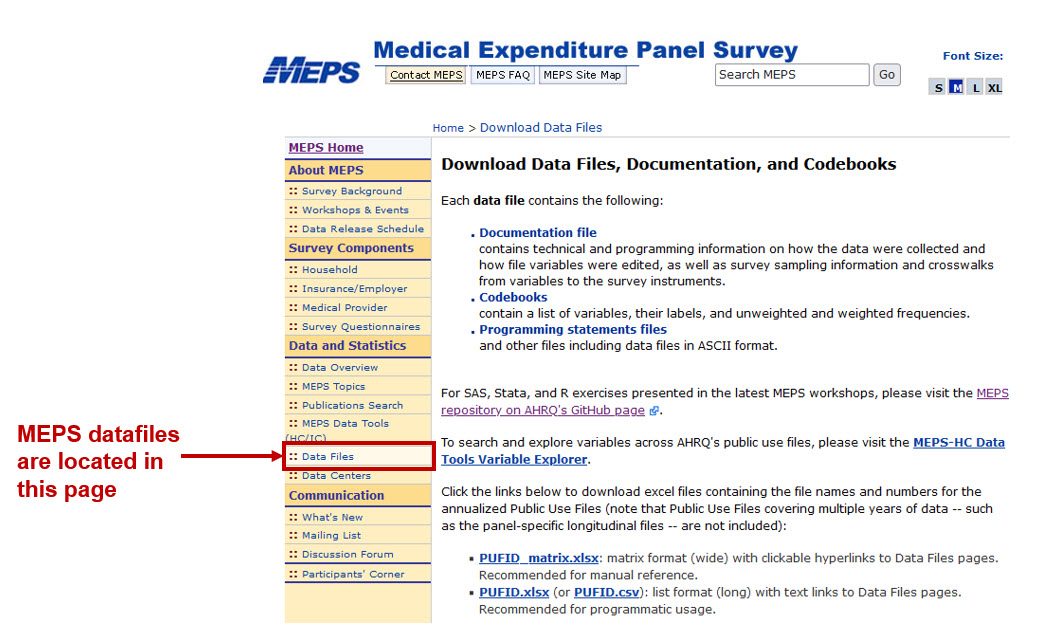
\includegraphics[width=1\linewidth]{Figure 1} \caption{Figure 1 - Location of MEPS data files}\label{fig:unnamed-chunk-2}
\end{figure}

The MEPS data files include the \href{https://www.meps.ahrq.gov/mepsweb/data_stats/download_data_files_detail.jsp?cboPufNumber=HC-224}{Full-Year Consolidated Data files}, which is the calendar-year summary of the different longitudinal panels. The Full-Year Consolidated Data files contain information on the annual healthcare expenditures by the type of care; it contains data on spending, insurance coverage, health status, patient satisfaction, and several health conditions. The Full-Year Consolidated Data files also contains information from several surveys (e.g,. Diabetes Care Survey).

\begin{figure}
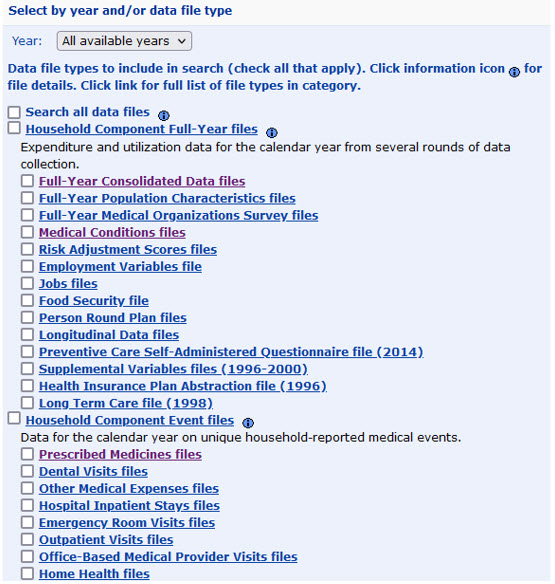
\includegraphics[width=1\linewidth]{Figure 2} \caption{Figure 2 - Full-Year Consolidated Data files and other data types}\label{fig:unnamed-chunk-3}
\end{figure}

\hypertarget{load-meps-data-into-r}{%
\section{Load MEPS data into R}\label{load-meps-data-into-r}}

MEPS data can be downloaded onto your local storage and read into a statistical software program such as Stata or R. But you can also communicate directly with the AHRQ MEPS website to load your data rather than having to download it. We will load the Full-Year Consolidated Data file from 2020, which is named \texttt{HC-224}. To find out the name of the file, you will need to go MEPS data files site and click on the Full-Year Consolidated Data files. In this page (Figure 2), you can see the data file with the code \texttt{HC-224}, which is the Full-Year Consolidated Data file for 2020. When we enter this into our R code, we will use the file name \texttt{h224}.

\begin{figure}
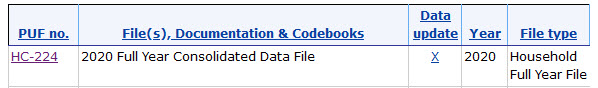
\includegraphics[width=1\linewidth]{Figure 3} \caption{Figure 3 - H224 is the MEP 2020 Full-Year Consolidated Data file.}\label{fig:unnamed-chunk-4}
\end{figure}

You will need to download and install the \href{https://github.com/e-mitchell/meps_r_pkg}{\texttt{MEPS} package}. The \texttt{MEPS} package will provide tools for you to load and manipulate the MEPS Data files. You will need to have R \texttt{devtools} package installed.

\begin{Shaded}
\begin{Highlighting}[]
\DocumentationTok{\#\# Install the devtools package}
\CommentTok{\# install.packages("devtools") \#\# You only need to install this once}
\CommentTok{\# library("devtools")  \#\# You will need to reload the MEPS package each time you restart R}
\CommentTok{\# install\_github("e{-}mitchell/meps\_r\_pkg/MEPS") \#\# This will install the MEPS package for R}
\end{Highlighting}
\end{Shaded}

There are two methods to load MEPS data into R.

Method 1 requires that you know the file name. In this example, the MEPS 2020 Full-Year Consolidated Data file is named \texttt{h224}. We will use the \texttt{read\_MEPS} function to load the MEPS data onto R.

When using Method 2 to load the MEPS data, we don't need to know the file name, but we need to know the year and the data type. For example, for the Full-Year Consolidated Data file, we use the \texttt{year\ =\ 2020} and \texttt{type\ =\ "FYC"} option. For this method, we will also use the \texttt{read\_MEPS} function to the MEPS data onto R.

The \texttt{tolower} function is used to change all the variable names from upper case to lower case. MEPS defaults the column names to upper case. I like to change this to lower case because it's easier for me to type.

\begin{Shaded}
\begin{Highlighting}[]
\DocumentationTok{\#\#\# Load the MEPS package}
\FunctionTok{library}\NormalTok{(}\StringTok{"MEPS"}\NormalTok{) }\DocumentationTok{\#\# You need to load the library every time you restart R}

\DocumentationTok{\#\#\#\# Method 1: Load data from AHRQ MEPS website}
\NormalTok{hc2020 }\OtherTok{=} \FunctionTok{read\_MEPS}\NormalTok{(}\AttributeTok{file =} \StringTok{"h224"}\NormalTok{)}

\DocumentationTok{\#\#\#\# Method 2: Load data from AHRQ MEPS website}
\NormalTok{hc2020 }\OtherTok{=} \FunctionTok{read\_MEPS}\NormalTok{(}\AttributeTok{year =} \DecValTok{2020}\NormalTok{, }\AttributeTok{type =} \StringTok{"FYC"}\NormalTok{)}

\DocumentationTok{\#\# Change column names to lowercase}
\FunctionTok{names}\NormalTok{(hc2020) }\OtherTok{\textless{}{-}} \FunctionTok{tolower}\NormalTok{(}\FunctionTok{names}\NormalTok{(hc2020))}
\end{Highlighting}
\end{Shaded}

There are over 1400 variables in the MEPS 2020 Full-Year Consolidated Data file. We can reduce this to the essential variables using the \texttt{subset} function. This will generate a smaller data frame that we will call \texttt{keep\_meps}. The variables that we want to collect are the subject unique identifier (\texttt{dupersid}), the survey weights (\texttt{varpsu}, \texttt{varstr}, \texttt{perwt20f}), and the total healthcare expenditures for 2020 (\texttt{totexp20}).

\begin{Shaded}
\begin{Highlighting}[]
\DocumentationTok{\#\#\# Keep the subject\textquotesingle{}s unique ID, survey weights, and total expenditures}
\NormalTok{keep\_meps }\OtherTok{\textless{}{-}} \FunctionTok{subset}\NormalTok{(hc2020, }\AttributeTok{select =} \FunctionTok{c}\NormalTok{(dupersid, varpsu, varstr, perwt20f, totexp20))}

\FunctionTok{head}\NormalTok{(keep\_meps) }\DocumentationTok{\#\# View the first six rows of the data frame}
\end{Highlighting}
\end{Shaded}

\begin{verbatim}
## # A tibble: 6 x 5
##   dupersid   varpsu varstr perwt20f totexp20
##   <chr>       <dbl>  <dbl>    <dbl>    <dbl>
## 1 2320005101      1   2079    8418.      459
## 2 2320005102      1   2079    5200.      564
## 3 2320006101      1   2028    2140.      140
## 4 2320006102      1   2028    2216.     4673
## 5 2320006103      1   2028    4157.      410
## 6 2320012102      2   2069    1961.     2726
\end{verbatim}

Since MEPS uses a complex survey design, these weights are needed to estimate standard errors that are reflective of the representative sample of the U.S. population. We'll learn how to apply these survey weights to the MEPS data files in a future tutorial.

\hypertarget{conclusions}{%
\section{Conclusions}\label{conclusions}}

Loading MEPS data into R allows us to perform analysis easily and quickly. In this tutorial, you learned how to load MEPS data into R directly from the MEPS website. However, you can also download the MEPS data onto your local storage and use the \texttt{setwd} command to set the working directory.

In future tutorials, we'll learn how to apply the survey weights and perform descriptive analyses using the MEPS data files.

\hypertarget{acknowledgements}{%
\section{Acknowledgements}\label{acknowledgements}}

There are a lot of tutorials on how to use MEPS data with R. I found the \href{https://github.com/HHS-AHRQ/MEPS}{AHRQ MEPS GitHub page} to be an invaluable resource.

This is a work in progress, and I may update this in the future.

\hypertarget{merging}{%
\chapter{Merging files}\label{merging}}

\hypertarget{introduction-1}{%
\section{Introduction}\label{introduction-1}}

We want to merge the Full-Year Consolidated Data file with the Medical Conditions file so that we can identify patients with a diagnosis of diabetes.

\hypertarget{load-meps-data}{%
\section{Load MEPS data}\label{load-meps-data}}

We need to lead the MEPS Full-Year Consolidated Data file and the Medical Conditions file from 2020. There are two methods to loading MEPS data into R. Method 1 requires you to know the name of the file. For example, the Medical Conditions file from 2020 is named \texttt{h222}. In Method 2, you need to know the \texttt{type\ =} of data you want to load. For example, the Medical Conditions file is named \texttt{CONDITIONS}.

I like to work with column names that are in the lower case, so I used the \texttt{tolower} function to change the column names from upper case to lower case.

\begin{Shaded}
\begin{Highlighting}[]
\DocumentationTok{\#\#\# Load the MEPS package}
\FunctionTok{library}\NormalTok{(}\StringTok{"MEPS"}\NormalTok{) }\DocumentationTok{\#\# You need to load the library every time you restart R}

\DocumentationTok{\#\#\#\# Method 1: Load data from AHRQ MEPS website}
\NormalTok{hc2020 }\OtherTok{=} \FunctionTok{read\_MEPS}\NormalTok{(}\AttributeTok{file =} \StringTok{"h224"}\NormalTok{)}
\NormalTok{mc2020 }\OtherTok{=} \FunctionTok{read\_MEPS}\NormalTok{(}\AttributeTok{file =} \StringTok{"h222"}\NormalTok{)}

\DocumentationTok{\#\#\#\# Method 2: Load data from AHRQ MEPS website}
\NormalTok{hc2020 }\OtherTok{=} \FunctionTok{read\_MEPS}\NormalTok{(}\AttributeTok{year =} \DecValTok{2020}\NormalTok{, }\AttributeTok{type =} \StringTok{"FYC"}\NormalTok{)}
\NormalTok{mc2020 }\OtherTok{=} \FunctionTok{read\_MEPS}\NormalTok{(}\AttributeTok{year =} \DecValTok{2020}\NormalTok{, }\AttributeTok{type =} \StringTok{"CONDITIONS"}\NormalTok{)}

\DocumentationTok{\#\# Change column names to lowercase}
\FunctionTok{names}\NormalTok{(hc2020) }\OtherTok{\textless{}{-}} \FunctionTok{tolower}\NormalTok{(}\FunctionTok{names}\NormalTok{(hc2020))}
\FunctionTok{names}\NormalTok{(mc2020) }\OtherTok{\textless{}{-}} \FunctionTok{tolower}\NormalTok{(}\FunctionTok{names}\NormalTok{(mc2020))}
\end{Highlighting}
\end{Shaded}

\hypertarget{merge-meps-data}{%
\section{Merge MEPS data}\label{merge-meps-data}}

Now that we have both the \texttt{h224} and \texttt{h222} file loaded into R, we can marge these files together. The Full-Year Consolidated Data file contains unique patients (e.g., each row is a unique patient); hence, the unique identifier \texttt{dupersid} is not repeatable. Figure 1 illustrates an example of a table with each row as a unique subject. Note how the \texttt{dupersid} does not repeat.

\begin{figure}
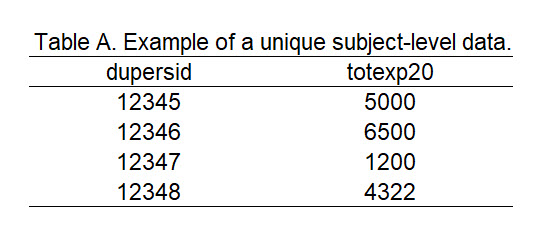
\includegraphics[width=0.8\linewidth]{Figure 2_1} \caption{Figure 1 - Example table with unique patients.}\label{fig:unnamed-chunk-9}
\end{figure}

However, in the Medical Conditions file, the rows are for the number of unique diagnosis grouped by the patient. In other words, the Medical Conditions file will contain repeated \texttt{dupersid} for each diagnosis. For example, a person can have 5 diagnosis grouped by their \texttt{dupersid}. In Figure 2, we have an example table with a subject \texttt{dupersid\ =\ 12345} who has five diagnosis (\texttt{icd10cdx}).

\begin{figure}
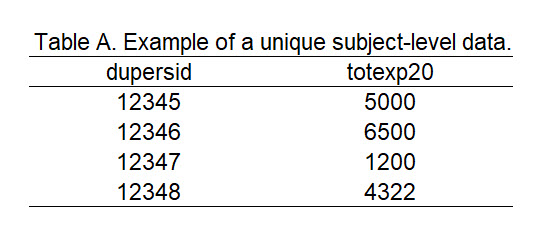
\includegraphics[width=1\linewidth]{Figure 2_1} \caption{Figure 2 - Example table where the unique patient identifier repeats.}\label{fig:unnamed-chunk-10}
\end{figure}

When we merge the Full-Year Consolidated Data file (which is unique to the \texttt{dupersid}) with the Medical Conditions file (which has repeatable \texttt{dupersid}), we will merge using a 1 to many merge (\texttt{Figure\ 3a}). \texttt{Figure\ 3a} illustrates the merge between the unique subject-level table to the repeatable subject-level table.

\begin{figure}
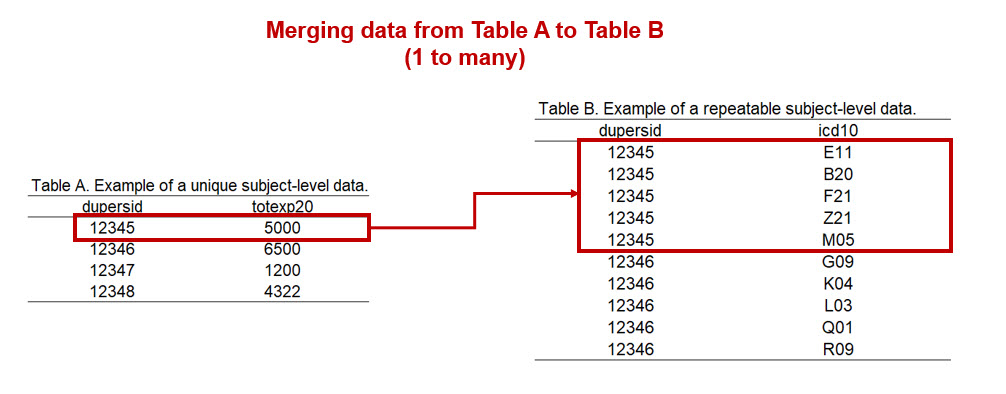
\includegraphics[width=1\linewidth]{Figure 2_3a} \caption{Figure 3a - Merging tables (1 to many).}\label{fig:unnamed-chunk-11}
\end{figure}

But we also want to make sure that we include all the patients in the Full-Year Consolidated Data file. Not all patients will have a diagnostic code, so we need to be careful that we don't accidentally drop them from the query. \texttt{Figure\ 3b} illustrates our intention to merge all the data from the Full-Year Consolidated Data file with some of the data from the Medical Conditions file.

\begin{figure}
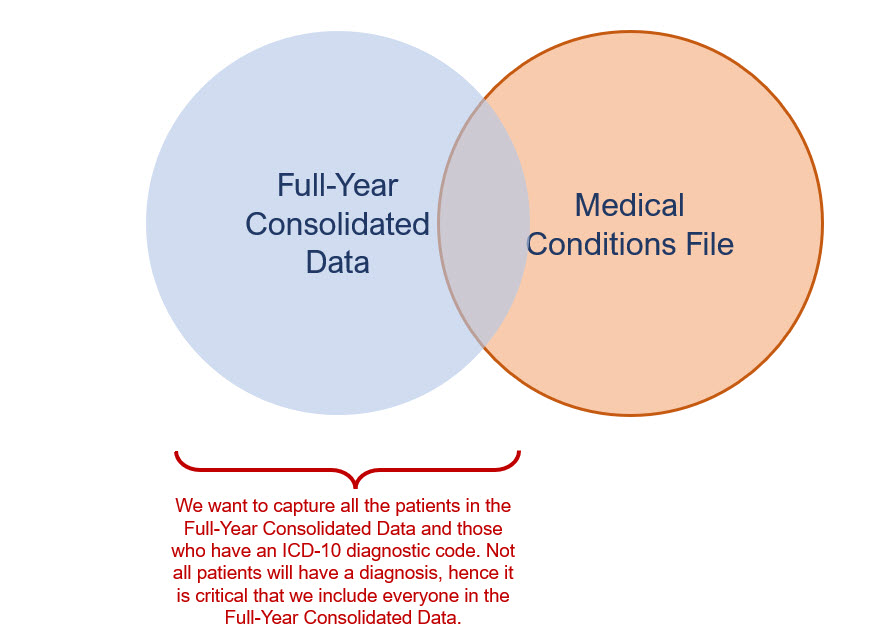
\includegraphics[width=1\linewidth]{Figure 2_3b} \caption{Figure 3b - Merging tables with all patients in the Full-Year Consolidated Data file and some of the data from the Medical Conditions file.}\label{fig:unnamed-chunk-12}
\end{figure}

Now that we understand how we want to merge the data, we can proceed to write the code.

There are two methods to merge the data files.

\textbf{Method 1:} We use the \texttt{merge} function to merge the two MEPS data files. The \texttt{by\ =} option is where we enter the matching variable \texttt{dupersid}. We will call the merged data set \texttt{total}. Using the `\texttt{merge} function, we are telling R that we want to do a 1 to many match between the Full-Year Consolidated Data file and the Medical Conditions file using the \texttt{dupersid} as the matching variable. We have to include the \texttt{all.x\ =\ TRUE} argument because we want to make sure we include the patients without any diagnostic codes.

\begin{Shaded}
\begin{Highlighting}[]
\DocumentationTok{\#\# MERGE data {-} Medical conditions and household component}
\CommentTok{\# merge two data frames by ID; there are two methods to do this:}

\DocumentationTok{\#\#\#\# Method 1: Native R function; Note: all.x means that we pull all dupersid, even the ones that don\textquotesingle{}t have a medical condition)}
\NormalTok{total }\OtherTok{\textless{}{-}} \FunctionTok{merge}\NormalTok{(hc2020, mc2020, }\AttributeTok{by =} \StringTok{"dupersid"}\NormalTok{, }\AttributeTok{all.x =} \ConstantTok{TRUE}\NormalTok{)}
\end{Highlighting}
\end{Shaded}

\textbf{Method 2:} We use the \texttt{left\_join} function from the \texttt{dplyr} package to merge the two MEPS data files. The \texttt{by\ =} option is where we enter the matching variable \texttt{dupersid}. We will call the merged data set \texttt{total}. Using the \texttt{left\_join} function, we are telling R that we want to do a 1 to many match between the Full-Year Consolidated Data file and the Medical Conditions file using the \texttt{dupersid} as the matching variable. The \texttt{left\_join} function is based on the SQL language syntax and operates in the same manner.

\begin{Shaded}
\begin{Highlighting}[]
\DocumentationTok{\#\#\#\# Method 2: Use SQL syntax (left\_join)}
\FunctionTok{library}\NormalTok{(}\StringTok{"dplyr"}\NormalTok{)}
\NormalTok{total }\OtherTok{\textless{}{-}} \FunctionTok{left\_join}\NormalTok{(hc2020, mc2020, }\AttributeTok{by =} \StringTok{"dupersid"}\NormalTok{)}
\end{Highlighting}
\end{Shaded}

Once the two data files are merged, we will have a data frame with repeatable \texttt{dupersid}. Notice that the \texttt{totexp20} variable from Table A is merged along with the \texttt{icd10} variable from Table B.

\begin{figure}
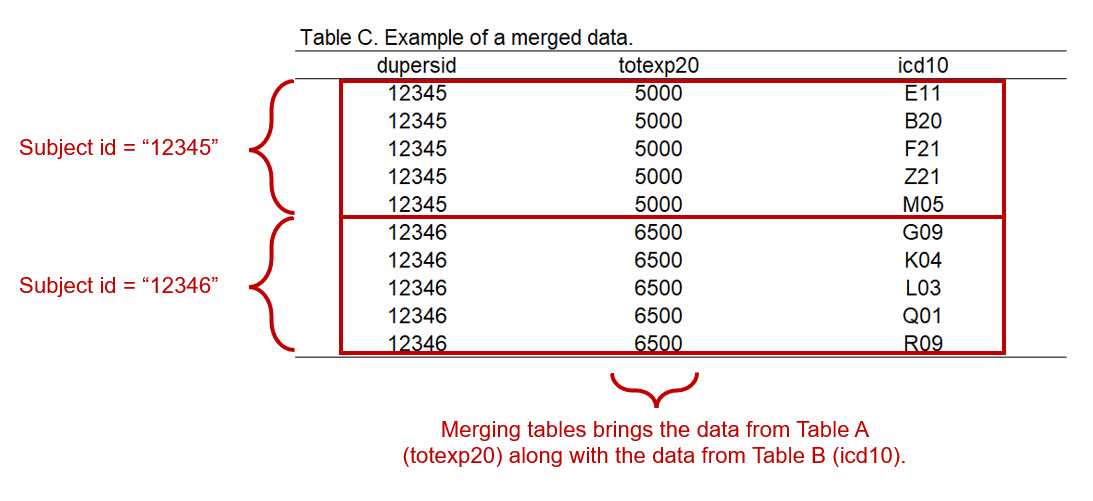
\includegraphics[width=1\linewidth]{Figure 2_4} \caption{Figure 4 - Merging data from Table A to Table B.}\label{fig:unnamed-chunk-15}
\end{figure}

\hypertarget{reduce-dataframe-to-a-few-variables}{%
\section{Reduce dataframe to a few variables}\label{reduce-dataframe-to-a-few-variables}}

Our \texttt{total} dataframe has 1481 variables and 80,802 observations. We want to make this dataframe manageable, so we'll create a limited dataframe with only the variables we're interested in. To do this, we'll use the \texttt{subset()} function.

For this exercise, we'll keep the \texttt{dupersid}, \texttt{varpsu.x}, \texttt{varsry.x}, \texttt{perwt20f.x}, and \texttt{icd10cdx} variables by using the \texttt{subset()} function. We'll call our reduced dataframe \texttt{keep\_mep2}. (Note: The \texttt{*.x} indicates the table on the left. We want to keep the \texttt{varpsu}, \texttt{varstr}, and \texttt{perwt20f} from the \texttt{hc2020} table. The \texttt{mc2020} table has duplicate variables that are denoted by \texttt{*.y}.)

\begin{Shaded}
\begin{Highlighting}[]
\NormalTok{keep\_meps2 }\OtherTok{\textless{}{-}} \FunctionTok{subset}\NormalTok{(total, }\AttributeTok{select =} \FunctionTok{c}\NormalTok{(}\StringTok{"dupersid"}\NormalTok{, }\StringTok{"varpsu.x"}\NormalTok{, }\StringTok{"varstr.x"}\NormalTok{, }\StringTok{"perwt20f.x"}\NormalTok{, }\StringTok{"icd10cdx"}\NormalTok{))}
\end{Highlighting}
\end{Shaded}

\hypertarget{add-an-indicator-for-a-specific-icd10-diagnostic-code}{%
\section{Add an indicator for a specific ICD10 diagnostic code}\label{add-an-indicator-for-a-specific-icd10-diagnostic-code}}

Our data frame has multiple rows grouped by the patient's id (\texttt{dupersid}); these rows are based on the various ICD-10 diagnostic codes. For example, patient \texttt{12345} has 5 ICD-10 diagnostic codes; hence, they have 5 rows (\texttt{Figure\ 4}).

Suppose we want to generate a binary indicator to identify patients with an ICD-10 diagnosis for diabetes (\texttt{E11}). In our example (\texttt{Figure\ 4}), patient \texttt{12345} has an ICD10 code for diabetes (\texttt{E11}).

We can create an indicator variable that will be unique to the patient for having diabetes. What we want to see if a new variable that identifies a patients with the specific ICD-10 code of interest. \texttt{Figure\ 5} illustrates the indicator variable for diabetes as an additional column \texttt{diabetes\_indicator}.

\begin{figure}
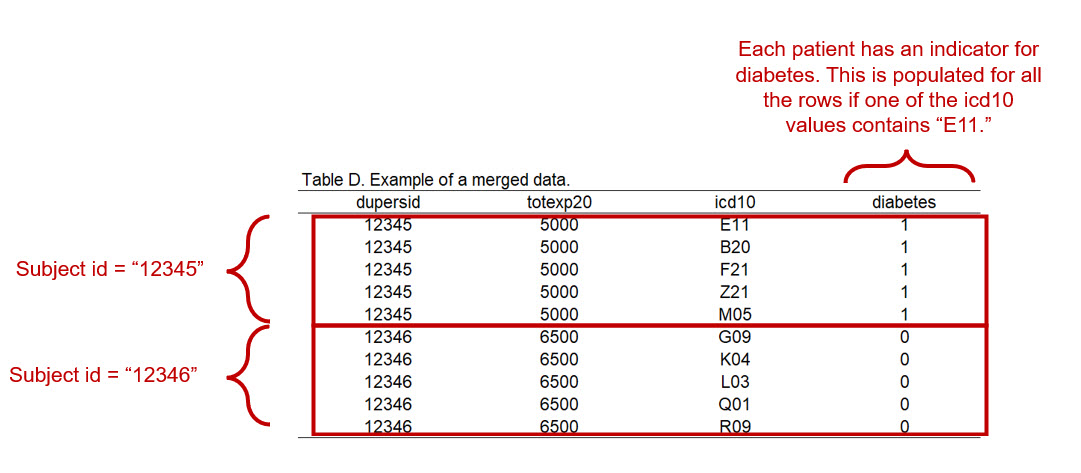
\includegraphics[width=1\linewidth]{Figure 2_5} \caption{Figure 5 - Indicator variable for diabetes.}\label{fig:unnamed-chunk-17}
\end{figure}

We create the indicator and call it \texttt{diabetes}, which is defined as \texttt{icd10cdx\ ==\ "E11"}. We will code this as \texttt{0} for no diabetes and \texttt{1} for diabetes. Then, we count the number of time a patient as \texttt{E11} in their \texttt{icd10cdx} column. I added the following option to the code (\texttt{\textbar{}\ is.na(total\$icd10cdx)}) because I want to make sure that all patients in the \texttt{total} table that do not have an ICD-10 code for \texttt{E11} is coded as \texttt{0}. There may be some patients that have \texttt{NA} or missing data in the \texttt{icd10cdx} variable. If the \texttt{icd10cdx} value is \texttt{NA}, this may not be coded with a \texttt{0}. Hence, we have to add the \texttt{\textbar{}\ is.na(total\$icd10cdx} code to ensure that we get a value of \texttt{0}.

\begin{Shaded}
\begin{Highlighting}[]
\DocumentationTok{\#\# Change to unique subject (each row is a unique subject)}
\DocumentationTok{\#\#\#\# Generate a variable to identify diabetes diagnosis for repeated rows}
\FunctionTok{library}\NormalTok{(}\StringTok{"tidyverse"}\NormalTok{)  }\DocumentationTok{\#\# Load tidyverse}

\NormalTok{keep\_meps2}\SpecialCharTok{$}\NormalTok{diabetes[total}\SpecialCharTok{$}\NormalTok{icd10cdx }\SpecialCharTok{!=} \StringTok{"E11"} \SpecialCharTok{|} \FunctionTok{is.na}\NormalTok{(total}\SpecialCharTok{$}\NormalTok{icd10cdx)] }\OtherTok{=} \DecValTok{0}
\NormalTok{keep\_meps2}\SpecialCharTok{$}\NormalTok{diabetes[total}\SpecialCharTok{$}\NormalTok{icd10cdx }\SpecialCharTok{==} \StringTok{"E11"}\NormalTok{] }\OtherTok{=} \DecValTok{1}

\FunctionTok{table}\NormalTok{(keep\_meps2}\SpecialCharTok{$}\NormalTok{diabetes) }\DocumentationTok{\#\# Visualize the number of patients with diabetes and no diabetes}
\end{Highlighting}
\end{Shaded}

\begin{verbatim}
## 
##     0     1 
## 87345  2693
\end{verbatim}

\begin{Shaded}
\begin{Highlighting}[]
\DocumentationTok{\#\#\# This code chunk calculates the number of times E11 appears for a unique patient}
\NormalTok{keep\_meps2 }\OtherTok{\textless{}{-}}\NormalTok{ keep\_meps2 }\SpecialCharTok{\%\textgreater{}\%}
  \FunctionTok{group\_by}\NormalTok{(dupersid) }\SpecialCharTok{\%\textgreater{}\%}
  \FunctionTok{mutate}\NormalTok{(}\AttributeTok{diabetes\_indicator =} \FunctionTok{sum}\NormalTok{(diabetes }\SpecialCharTok{==} \StringTok{"1"}\NormalTok{, }\AttributeTok{na.rm =} \ConstantTok{TRUE}\NormalTok{)) }\SpecialCharTok{\%\textgreater{}\%}
\NormalTok{  ungroup}
\FunctionTok{table}\NormalTok{(keep\_meps2}\SpecialCharTok{$}\NormalTok{diabetes\_indicator)}
\end{Highlighting}
\end{Shaded}

\begin{verbatim}
## 
##     0     1     2 
## 71804 17295   939
\end{verbatim}

According to our results, there were 17,295 events where a patient had one diagnostic code for \texttt{E11} and 939 events where a patient had two diagnostic codes for \texttt{E11}. How did this occur? MEPS public files only list the first three digits of the ICD-10 code to protect the identity of the patient. The ICD-10 diagnostic code has more digits beyond the first three. For example, an ICD-10 diagnosis for Type 2 diabetes with diabetic chronic kidney disease is \texttt{E11.22}. Hence, there will be patients with unique ICD-10 codes that may appear identical because only the first three digits are present in the MEPS public files.

In our example, we have patients with 1 and 2 ICD-10 diagnostic codes for \texttt{E11}. We would like to create a binary indicator of diabetes, so we need to take the current information and transform the variable \texttt{diabetes} in the \texttt{keep\_meps} dataframe into a new variable that only has \texttt{0} and \texttt{1}.

We can do this by combining the \texttt{mutate} function with the \texttt{ifelse} function. See the code below:

\begin{Shaded}
\begin{Highlighting}[]
\NormalTok{keep\_meps2 }\OtherTok{\textless{}{-}}\NormalTok{ keep\_meps2 }\SpecialCharTok{\%\textgreater{}\%} 
  \FunctionTok{group\_by}\NormalTok{(dupersid) }\SpecialCharTok{\%\textgreater{}\%}
  \FunctionTok{mutate}\NormalTok{(}\AttributeTok{diabetes\_binary =} \FunctionTok{ifelse}\NormalTok{(diabetes\_indicator }\SpecialCharTok{\textgreater{}=} \DecValTok{1}\NormalTok{, }\DecValTok{1}\NormalTok{, }\DecValTok{0}\NormalTok{), }\AttributeTok{na.rm =} \ConstantTok{TRUE}\NormalTok{) }\SpecialCharTok{\%\textgreater{}\%}
\NormalTok{  ungroup}
\FunctionTok{table}\NormalTok{(keep\_meps2}\SpecialCharTok{$}\NormalTok{diabetes\_binary)}
\end{Highlighting}
\end{Shaded}

\begin{verbatim}
## 
##     0     1 
## 71804 18234
\end{verbatim}

Now, we have a new binary indicator variable. The \texttt{diabetes\_binary} variable is coded \texttt{1} if the patient has the \texttt{E11} diagnostic code and \texttt{0} if the patient does not.

\hypertarget{collapse-dataframe-to-a-single-unique-patient}{%
\section{Collapse dataframe to a single unique patient}\label{collapse-dataframe-to-a-single-unique-patient}}

But since this is a dataframe with duplicated patients, we want to collapse this into a dataframe where each row is a single unique patient.

Since a lot of the variables in the dataframe are the same when grouped by the unique \texttt{dupersid}, we can estimate the mean and get the same value. For example, let's look at \texttt{Figure\ 5} again. For \texttt{dupersid\ ==\ 12345}, there are five values for \texttt{totexp20}, which are:

\begin{itemize}
\item
  \texttt{5000} when \texttt{icd10} is \texttt{E11},
\item
  \texttt{5000} when \texttt{icd10} is \texttt{B20},
\item
  \texttt{5000} when \texttt{icd10} is \texttt{F21},
\item
  \texttt{5000} when \texttt{icd10} is \texttt{Z21}, and
\item
  \texttt{5000} when \texttt{icd10} is \texttt{M05}
\end{itemize}

Averaging the \texttt{totexp20} for \texttt{dupersid\ ==\ 12345} will result in a value of \texttt{5000}.

Hence, when we average the diabetes \texttt{diabetes\_binary} variable, we will get a value of \texttt{1} or \texttt{0}.

Using this knowledge, we can collapse our data to a single \texttt{dupersid} and remove the duplicates.

The \texttt{icd10cdx} variable will yielded \texttt{NA} because it can't be collapsed numerically due to its \texttt{string} data type.

\(~\)

There are two methods to collapse the dataframe to unique patients:

\textbf{Method 1:} Use the \texttt{dplyr} package and the \texttt{summarize\_all} function with the \texttt{list()} function.

\begin{Shaded}
\begin{Highlighting}[]
\DocumentationTok{\#\#\#\# Collapse the repeated rows to a single unique subject}
\NormalTok{meps\_per }\OtherTok{\textless{}{-}}\NormalTok{ keep\_meps2 }\SpecialCharTok{\%\textgreater{}\%} 
  \FunctionTok{group\_by}\NormalTok{(dupersid) }\SpecialCharTok{\%\textgreater{}\%}
  \FunctionTok{summarize\_all}\NormalTok{(}\FunctionTok{list}\NormalTok{(mean))}

\FunctionTok{table}\NormalTok{(meps\_per}\SpecialCharTok{$}\NormalTok{diabetes\_binary)}
\end{Highlighting}
\end{Shaded}

\begin{verbatim}
## 
##     0     1 
## 25202  2603
\end{verbatim}

\(~\)

\textbf{Method 2:} Use the \texttt{summarise} function. This method will generate a dataframe with two variables (\texttt{dupersid} and \texttt{diabetes\_binary2}).

\begin{Shaded}
\begin{Highlighting}[]
\NormalTok{meps\_per2 }\OtherTok{\textless{}{-}}\NormalTok{ keep\_meps2 }\SpecialCharTok{\%\textgreater{}\%}  \DocumentationTok{\#\#\# An alternative method but only generates two variables (dupersid and diabetes\_binary2)}
  \FunctionTok{group\_by}\NormalTok{(dupersid) }\SpecialCharTok{\%\textgreater{}\%}
  \FunctionTok{summarise}\NormalTok{(}\AttributeTok{diabetes\_binary2 =} \FunctionTok{mean}\NormalTok{(diabetes\_binary)) }\SpecialCharTok{\%\textgreater{}\%}
  \FunctionTok{as.data.frame}\NormalTok{()}

\FunctionTok{table}\NormalTok{(meps\_per2}\SpecialCharTok{$}\NormalTok{diabetes\_binary2)}
\end{Highlighting}
\end{Shaded}

\begin{verbatim}
## 
##     0     1 
## 25202  2603
\end{verbatim}

For the rest of the tutorial, I'll use Method 1 because I want to keep the other variables.

\texttt{Figure\ 6} illustrates what our dataframe should look like after we collapsed the data to a single unique patient.

\begin{figure}
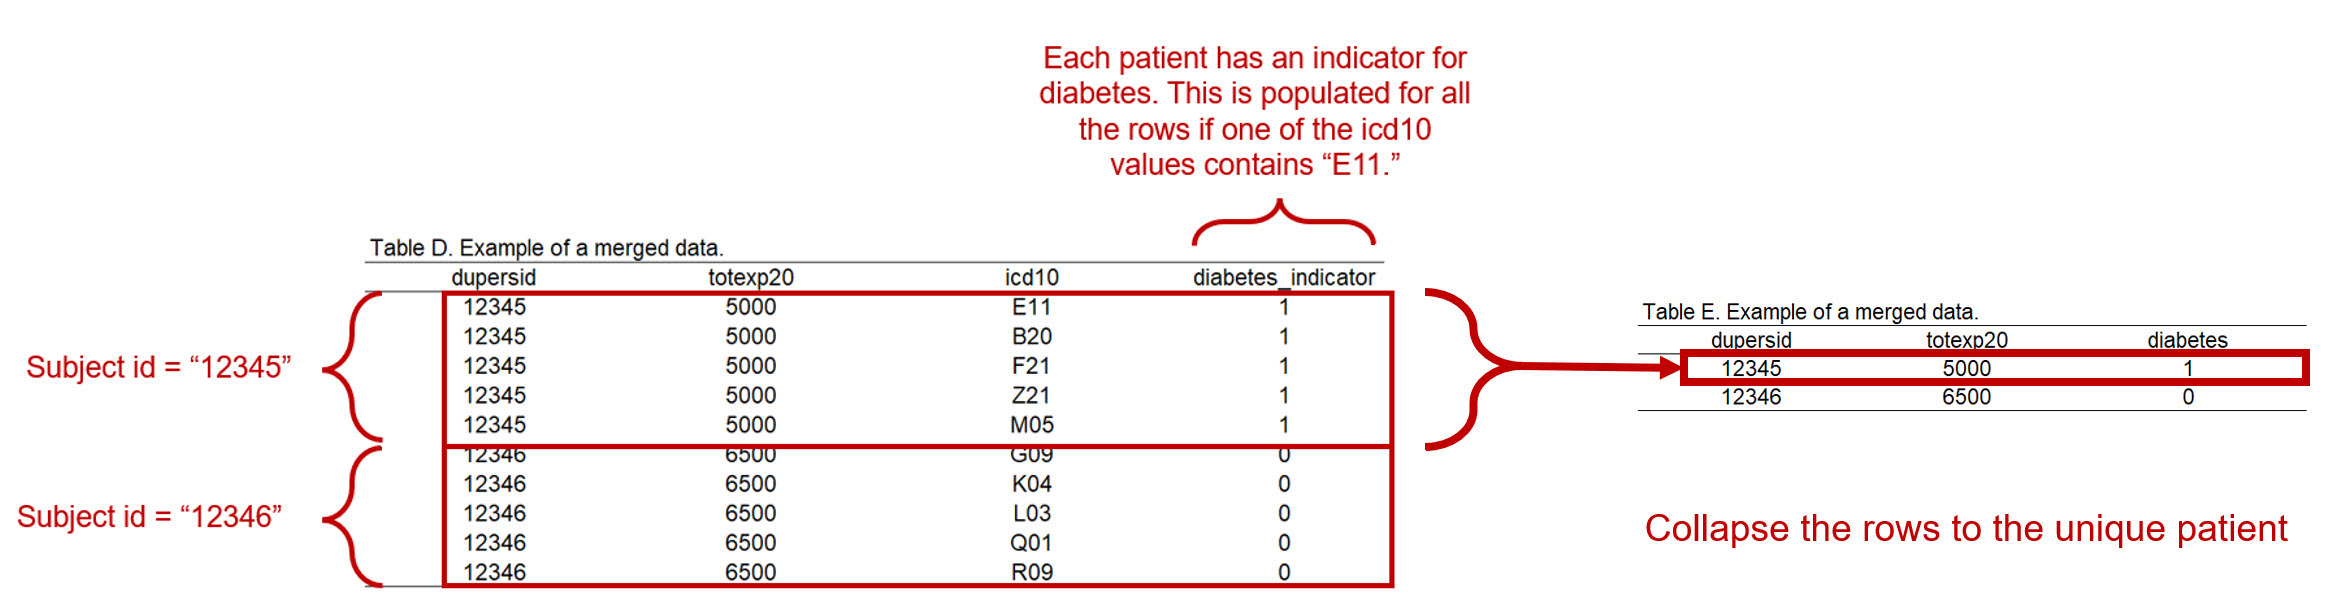
\includegraphics[width=1\linewidth]{Figure 2_6} \caption{Figure 6 - Collapse rows to a unique patient with a diabetes indicator.}\label{fig:unnamed-chunk-22}
\end{figure}

\hypertarget{conclusions-1}{%
\section{Conclusions}\label{conclusions-1}}

With this tutorial, we've learned how to merge two data files from MEPS and collapse them to a dataframe of unique patients. MEPS has additional data files that contain information that might be important for your work. For example, we can use these methods to merge the Prescription Drug file and create indicators for patients who are on opioids. However, you will need to carefully read through the documentation for each data file to understand what kind of information they contain. Feel free to explore using these strategies to merge additional MEPS data files to your existing cohort.

\hypertarget{acknowledgements-1}{%
\section{Acknowledgements}\label{acknowledgements-1}}

There are a lot of tutorials on how to use MEPS data with R. I found the \href{https://github.com/HHS-AHRQ/MEPS}{AHRQ MEPS GitHub page} to be an invaluable resource.

\href{https://daranzolin.github.io/}{David Ranzolin} has a great \href{https://rstudio-pubs-static.s3.amazonaws.com/116317_e6922e81e72e4e3f83995485ce686c14.html\#/2}{presentation} on how to use the \texttt{mutate} function in R. I liked the examples he used, and the presentation is succint and informative.

Another great resource is by \href{https://statisticsglobe.com/joachim-schork/}{Joachim Schork}, author and founder of \href{https://statisticsglobe.com/}{Statistics Globe} who wrote a great \href{https://statisticsglobe.com/sum-duplicate-rows-r}{blog} about collapsing data on a unique identifier.

I learned how to use the \texttt{left\_join} function from this \href{https://www.infoworld.com/article/3454356/how-to-merge-data-in-r-using-r-merge-dplyr-or-datatable.html}{blog} by \href{https://www.infoworld.com/author/Sharon-Machlis/}{Sharon Machlis} on \href{https://www.infoworld.com}{InfoWorld}. She uses \texttt{dplyr} to invoke the \texttt{left\_join} function which is a based on \texttt{SQL} language.

This is a work in progress, and I may update this in the future.

\hypertarget{weights}{%
\chapter{Applying weights}\label{weights}}

\hypertarget{introduction-2}{%
\section{Introduction}\label{introduction-2}}

The \href{https://www.meps.ahrq.gov/mepsweb/}{Medical Expenditure Panel Survey (MEPS)} is based on a complex survey design. Hence, it is necessary to apply survey weights to generate estimates that are representative of the United States (US) population. The weights take into account the stratification, clustering, sampling, and non-response based on the Current Population Survey. Although you can perform descriptive and complex analyses without the weights, they will not provide you with accurate standard errors of the population. Rather, not applying the weights will only yield standard errors for the sample.

\hypertarget{types-of-weights}{%
\section{Types of weights}\label{types-of-weights}}

In MEPS, there are three types of weights that are critical for most descriptive and multivariate analyses: person weight (\texttt{perwtXXf}), stratum (\texttt{varstr}), and cluster (\texttt{varpsu}). The \texttt{XX} is replaced by the year of the survey. For example, the person weight in 2020 is labelled as \texttt{perwt20f}.

\hypertarget{loading-the-data}{%
\section{Loading the data}\label{loading-the-data}}

Let's use the MEPS Full-Year Consolidated File from 2020. From our previous tutorial, you can load data using the \texttt{MEPS} library function \texttt{read\_MEPS}. There are two methods that you can use to load data into R.

\begin{Shaded}
\begin{Highlighting}[]
\DocumentationTok{\#\#\# Load the MEPS package}
\FunctionTok{library}\NormalTok{(}\StringTok{"MEPS"}\NormalTok{) }\DocumentationTok{\#\# You need to load the library every time you restart R}

\DocumentationTok{\#\#\#\# Method 1: Load data from AHRQ MEPS website}
\NormalTok{hc2020 }\OtherTok{=} \FunctionTok{read\_MEPS}\NormalTok{(}\AttributeTok{file =} \StringTok{"h224"}\NormalTok{)}

\DocumentationTok{\#\#\#\# Method 2: Load data from AHRQ MEPS website}
\NormalTok{hc2020 }\OtherTok{=} \FunctionTok{read\_MEPS}\NormalTok{(}\AttributeTok{year =} \DecValTok{2020}\NormalTok{, }\AttributeTok{type =} \StringTok{"FYC"}\NormalTok{)}

\DocumentationTok{\#\# Change column names to lowercase}
\FunctionTok{names}\NormalTok{(hc2020) }\OtherTok{\textless{}{-}} \FunctionTok{tolower}\NormalTok{(}\FunctionTok{names}\NormalTok{(hc2020))}
\end{Highlighting}
\end{Shaded}

Once the data has been loaded, we can look at how many variables there are.

\begin{Shaded}
\begin{Highlighting}[]
\DocumentationTok{\#\# The number of columns represents the number of variables in the hc2020 dataframe. }
\FunctionTok{ncol}\NormalTok{(hc2020)}
\end{Highlighting}
\end{Shaded}

\begin{verbatim}
## [1] 1451
\end{verbatim}

We have over 1400 variable. This is a very large dataframe. We can reduce this to a manageable size by keeping only the variables that are important. Let's keep the unique patient identifier (\texttt{dupersid}), weights (\texttt{perwt20f}, \texttt{varstr}, and \texttt{varpsu}), and the total expenditures (\texttt{totexp20}).

\begin{Shaded}
\begin{Highlighting}[]
\DocumentationTok{\#\# Create a smaller dataframe}
\NormalTok{keep\_hc2020 }\OtherTok{\textless{}{-}} \FunctionTok{subset}\NormalTok{(hc2020, }\AttributeTok{select =} \FunctionTok{c}\NormalTok{(dupersid, perwt20f, varstr, varpsu, totexp20, sex, povcat20))}
\FunctionTok{head}\NormalTok{(keep\_hc2020)}
\end{Highlighting}
\end{Shaded}

\begin{verbatim}
## # A tibble: 6 x 7
##   dupersid   perwt20f varstr varpsu totexp20 sex          povcat20           
##   <chr>         <dbl>  <dbl>  <dbl>    <dbl> <dbl+lbl>    <dbl+lbl>          
## 1 2320005101    8418.   2079      1      459 2 [2 FEMALE] 2 [2 NEAR POOR]    
## 2 2320005102    5200.   2079      1      564 1 [1 MALE]   2 [2 NEAR POOR]    
## 3 2320006101    2140.   2028      1      140 2 [2 FEMALE] 3 [3 LOW INCOME]   
## 4 2320006102    2216.   2028      1     4673 1 [1 MALE]   1 [1 POOR/NEGATIVE]
## 5 2320006103    4157.   2028      1      410 1 [1 MALE]   3 [3 LOW INCOME]   
## 6 2320012102    1961.   2069      2     2726 2 [2 FEMALE] 3 [3 LOW INCOME]
\end{verbatim}

We can add labels to the \texttt{sex} variable where \texttt{1\ =\ male} and \texttt{2\ =\ female}.

\hypertarget{perform-descriptive-analysis}{%
\section{Perform descriptive analysis}\label{perform-descriptive-analysis}}

Now that we have a smaller dataframe with the variables of interest, let's apply the survey weights to some descriptive analysis.

Suppose you were interested in the average age of the cohort. You will need to apply the survey weights to generate the mean and standard deviation. The \texttt{survey} package comes with the \texttt{svydesign} function, which uses the survey weights in the Full-Year Consolidated File data and applies them to the cohort in preparation for analyses.

First, you will need to set the options to \texttt{adjust}, which centers the single-PSU strata arund the grand mean rather than the stratum mean. With MEPS data, we are using single-PSU (or ``lonely'' PSU), which is used to estimate the variance by calculating the difference of the sum of the statum's PSU and the average statum's PSU. The, we use the \texttt{svydesign} function to generate a complex survey design dataset (which we will call \texttt{mepsdsgn}) for analysis by applying the survey weights.

\begin{Shaded}
\begin{Highlighting}[]
\DocumentationTok{\#\# Load the "survey" package}
\FunctionTok{library}\NormalTok{(}\StringTok{"survey"}\NormalTok{)}

\DocumentationTok{\#\# Apply the survey weights to the dataframe using the svydesign function}
\FunctionTok{options}\NormalTok{(}\AttributeTok{survey.lonely.psu =} \StringTok{\textquotesingle{}adjust\textquotesingle{}}\NormalTok{)}

\NormalTok{mepsdsgn }\OtherTok{=} \FunctionTok{svydesign}\NormalTok{(}
  \AttributeTok{id =} \SpecialCharTok{\textasciitilde{}}\NormalTok{varpsu,}
  \AttributeTok{strata =} \SpecialCharTok{\textasciitilde{}}\NormalTok{varstr,}
  \AttributeTok{weights =} \SpecialCharTok{\textasciitilde{}}\NormalTok{perwt20f,}
  \AttributeTok{data =}\NormalTok{ keep\_hc2020,}
  \AttributeTok{nest =} \ConstantTok{TRUE}\NormalTok{)}
\end{Highlighting}
\end{Shaded}

Once the survey weights have been applied, we can use the \texttt{survey} functions to perform some descriptive analysis on the \texttt{mepsdsgn} data.

First, let's see how many patients we have that is representative of the US population by sex. We use the \texttt{svytable} function to generate the weight sample for males and females. Adding these together will yield the weighted sample of the US population.

\begin{Shaded}
\begin{Highlighting}[]
\DocumentationTok{\#\# Weighted sample of the population stratified by sex}
\FunctionTok{svytable}\NormalTok{(}\SpecialCharTok{\textasciitilde{}}\NormalTok{sex, }\AttributeTok{design =}\NormalTok{ mepsdsgn)}
\end{Highlighting}
\end{Shaded}

\begin{verbatim}
## sex
##   1 - Male 2 - Female 
##  160960989  167584308
\end{verbatim}

Using the survey weights, there are 160,960,989 males and 167,584,308 females. In total, there are 328,545,297 weighted subjects in the \texttt{mepsdsgn} data.

Let's move on and estimate the average total expenditures for the total sample.

\begin{Shaded}
\begin{Highlighting}[]
\DocumentationTok{\#\# Estimate the weighted mean total expenditure for the sample}
\FunctionTok{svymean}\NormalTok{(}\SpecialCharTok{\textasciitilde{}}\NormalTok{totexp20, }\AttributeTok{design =}\NormalTok{ mepsdsgn)}
\end{Highlighting}
\end{Shaded}

\begin{verbatim}
##            mean     SE
## totexp20 6266.1 164.38
\end{verbatim}

The \texttt{svymean} function generates the appropriate average and standard error (SE) of the total sample that is representative of the US population. In 2020, the average total expenditure was \$6266 (SE, 164).

In our \texttt{mepsdsgn} data, we have sex, which is a binary variable. Let's estimate the total expenditures between males and females in the MEPS Full-Year Consolidated data. To estimate the mean between two groups, we'll need to use the \texttt{svyby} function along with the \texttt{svymean} function.

\begin{Shaded}
\begin{Highlighting}[]
\DocumentationTok{\#\# Estimate the weight mean total expenditure for males and females}
\FunctionTok{svyby}\NormalTok{(}\SpecialCharTok{\textasciitilde{}}\NormalTok{totexp20, }\SpecialCharTok{\textasciitilde{}}\NormalTok{sex, mepsdsgn, svymean)}
\end{Highlighting}
\end{Shaded}

\begin{verbatim}
##                   sex totexp20       se
## 1 - Male     1 - Male 5861.278 243.5624
## 2 - Female 2 - Female 6654.998 205.0776
\end{verbatim}

The average total expenditures for male and female are \$5861 (SE, 244) and \$6655 (SE 205), respectively.

We can perform crosstabulations with the \texttt{svytable} function. Let's look at the distribution of males and females across various poverty categories. In the MEPS codebook, poverty category are groups as: 1 = Poor/Negative, 2 = Near Poor, 3 = Low Income, 4 = Middle Income, and 5 = High Income.

\begin{Shaded}
\begin{Highlighting}[]
\DocumentationTok{\#\# Crosstab sex and poverty category}
\FunctionTok{svytable}\NormalTok{(}\SpecialCharTok{\textasciitilde{}}\NormalTok{sex }\SpecialCharTok{+}\NormalTok{ povcat20, }\AttributeTok{design =}\NormalTok{ mepsdsgn)}
\end{Highlighting}
\end{Shaded}

\begin{verbatim}
##             povcat20
## sex                 1        2        3        4        5
##   1 - Male   16644995  5955576 18910001 45083571 74366846
##   2 - Female 21002826  6672752 21753502 47750327 70404901
\end{verbatim}

To generate the proportions, you will need to use \texttt{prop.table}. We add the \texttt{margin\ =\ 1} option to calculate the column total.

\begin{Shaded}
\begin{Highlighting}[]
\FunctionTok{prop.table}\NormalTok{(}\FunctionTok{svytable}\NormalTok{(}\SpecialCharTok{\textasciitilde{}}\NormalTok{sex }\SpecialCharTok{+}\NormalTok{ povcat20, }\AttributeTok{design =}\NormalTok{ mepsdsgn), }\AttributeTok{margin =} \DecValTok{1}\NormalTok{) }\DocumentationTok{\#\#\# margin = 1 calculates the column total.}
\end{Highlighting}
\end{Shaded}

\begin{verbatim}
##             povcat20
## sex                   1          2          3          4          5
##   1 - Male   0.10341012 0.03700012 0.11748189 0.28009005 0.46201783
##   2 - Female 0.12532693 0.03981729 0.12980632 0.28493316 0.42011631
\end{verbatim}

We can combine these into a contingency table using the \texttt{tbl\_svysummary} function from the \texttt{gtsummary} package. We will also use the \texttt{tidyverse} package to manipulate the data more easily.

\begin{Shaded}
\begin{Highlighting}[]
\DocumentationTok{\#\# Load libraries }
\FunctionTok{library}\NormalTok{(}\StringTok{"tidyverse"}\NormalTok{)}
\FunctionTok{library}\NormalTok{(}\StringTok{"gtsummary"}\NormalTok{)}

\DocumentationTok{\#\# Contingency table (crosstabulations between sex and poverty category)}
\NormalTok{mepsdsgn }\SpecialCharTok{\%\textgreater{}\%}
  \FunctionTok{tbl\_svysummary}\NormalTok{(}\AttributeTok{by =}\NormalTok{ sex, }\AttributeTok{percent =} \StringTok{"column"}\NormalTok{, }\AttributeTok{include =} \FunctionTok{c}\NormalTok{(povcat20))}
\end{Highlighting}
\end{Shaded}

\begin{tabular}{l|c|c}
\hline
**Characteristic** & **1 - Male**, N = 160,960,989 & **2 - Female**, N = 167,584,308\\
\hline
FAMILY INC AS \% OF POVERTY LINE - CATEGORICAL &  & \\
\hline
1 & 16,644,995 (10\%) & 21,002,826 (13\%)\\
\hline
2 & 5,955,576 (3.7\%) & 6,672,752 (4.0\%)\\
\hline
3 & 18,910,001 (12\%) & 21,753,502 (13\%)\\
\hline
4 & 45,083,571 (28\%) & 47,750,327 (28\%)\\
\hline
5 & 74,366,846 (46\%) & 70,404,901 (42\%)\\
\hline
\end{tabular}

Based on these weighted sample numbers, there are more males who are in the High Income category compared to females (46\% versus 42\%).

\hypertarget{conclusions-2}{%
\section{Conclusions}\label{conclusions-2}}

The MEPS data uses weights to generate estimations that are reflective of the US population. The \texttt{survey} package from R will allow us to apply these weights using the \texttt{svydesign} function, which requires us to enter the patient weight, stratum, and cluster values. Once these are applied, we can use the suite of functions from the \texttt{survey} package to perform descriptive analysis on the population. The \texttt{svymean} generates the population average and the \texttt{svytable} generates the population frequencies. Having a good understanding of how these weights are used with MEPS data will allow you to generate estimates of the population in your epidemiology work.

\hypertarget{acknowledgements-2}{%
\section{Acknowledgements}\label{acknowledgements-2}}

The \texttt{survey} package and functions were developed by \href{https://profiles.auckland.ac.nz/t-lumley}{Thomas Lumley} and can be found \href{https://www.rdocumentation.org/packages/survey/versions/4.1-1}{here}.

The \texttt{gtsummary} package and instructions are developed by Daniel D. Sjoberg, Joseph Larmarange, Michael Curry, Jessica Lavery, Karissa Whiting, Emily C. Zabor, which can be found at their \href{https://www.danieldsjoberg.com/gtsummary/reference/tbl_svysummary.html}{website}.

This is a work in progress, and I expect to make updates in the future.

\hypertarget{footnotes-and-citations}{%
\chapter{Footnotes and citations}\label{footnotes-and-citations}}

\hypertarget{footnotes}{%
\section{Footnotes}\label{footnotes}}

Footnotes are put inside the square brackets after a caret \texttt{\^{}{[}{]}}. Like this one \footnote{This is a footnote.}.

\hypertarget{citations}{%
\section{Citations}\label{citations}}

Reference items in your bibliography file(s) using \texttt{@key}.

For example, we are using the \textbf{bookdown} package \citep{R-bookdown} (check out the last code chunk in index.Rmd to see how this citation key was added) in this sample book, which was built on top of R Markdown and \textbf{knitr} \citep{xie2015} (this citation was added manually in an external file book.bib).
Note that the \texttt{.bib} files need to be listed in the index.Rmd with the YAML \texttt{bibliography} key.

The RStudio Visual Markdown Editor can also make it easier to insert citations: \url{https://rstudio.github.io/visual-markdown-editing/\#/citations}

\hypertarget{blocks}{%
\chapter{Blocks}\label{blocks}}

\hypertarget{equations}{%
\section{Equations}\label{equations}}

Here is an equation.

\begin{equation} 
  f\left(k\right) = \binom{n}{k} p^k\left(1-p\right)^{n-k}
  \label{eq:binom}
\end{equation}

You may refer to using \texttt{\textbackslash{}@ref(eq:binom)}, like see Equation \eqref{eq:binom}.

\hypertarget{theorems-and-proofs}{%
\section{Theorems and proofs}\label{theorems-and-proofs}}

Labeled theorems can be referenced in text using \texttt{\textbackslash{}@ref(thm:tri)}, for example, check out this smart theorem \ref{thm:tri}.

\begin{theorem}
\protect\hypertarget{thm:tri}{}\label{thm:tri}For a right triangle, if \(c\) denotes the \emph{length} of the hypotenuse
and \(a\) and \(b\) denote the lengths of the \textbf{other} two sides, we have
\[a^2 + b^2 = c^2\]
\end{theorem}

Read more here \url{https://bookdown.org/yihui/bookdown/markdown-extensions-by-bookdown.html}.

\hypertarget{callout-blocks}{%
\section{Callout blocks}\label{callout-blocks}}

The R Markdown Cookbook provides more help on how to use custom blocks to design your own callouts: \url{https://bookdown.org/yihui/rmarkdown-cookbook/custom-blocks.html}

\hypertarget{sharing-your-book}{%
\chapter{Sharing your book}\label{sharing-your-book}}

\hypertarget{publishing}{%
\section{Publishing}\label{publishing}}

HTML books can be published online, see: \url{https://bookdown.org/yihui/bookdown/publishing.html}

\hypertarget{pages}{%
\section{404 pages}\label{pages}}

By default, users will be directed to a 404 page if they try to access a webpage that cannot be found. If you'd like to customize your 404 page instead of using the default, you may add either a \texttt{\_404.Rmd} or \texttt{\_404.md} file to your project root and use code and/or Markdown syntax.

\hypertarget{metadata-for-sharing}{%
\section{Metadata for sharing}\label{metadata-for-sharing}}

Bookdown HTML books will provide HTML metadata for social sharing on platforms like Twitter, Facebook, and LinkedIn, using information you provide in the \texttt{index.Rmd} YAML. To setup, set the \texttt{url} for your book and the path to your \texttt{cover-image} file. Your book's \texttt{title} and \texttt{description} are also used.

This \texttt{gitbook} uses the same social sharing data across all chapters in your book- all links shared will look the same.

Specify your book's source repository on GitHub using the \texttt{edit} key under the configuration options in the \texttt{\_output.yml} file, which allows users to suggest an edit by linking to a chapter's source file.

Read more about the features of this output format here:

\url{https://pkgs.rstudio.com/bookdown/reference/gitbook.html}

Or use:

\begin{Shaded}
\begin{Highlighting}[]
\NormalTok{?bookdown}\SpecialCharTok{::}\NormalTok{gitbook}
\end{Highlighting}
\end{Shaded}


  \bibliography{book.bib,packages.bib}

\end{document}
